\subsection{Pattern di gestione dello stato}\label{subsec:state-manage}
Durante la fase di progettazione di un sistema software, è fondamentale definire la struttura con la quale le singole componenti saranno organizzate.

Nel contesto applicativo di software orientati all'interazione con l'utente tramite interfaccia grafica, come ad esempio un'applicazione web,
è spesso consigliato definire chiaramente la gestione dello stato e del flusso informativo, quando questi non sono imposti da eventuali framework utilizzati.

Per esempio, come accennato nella~\Cref{subsec:react}, React prevede che la struttura dei componenti sia definita da un albero:
lo stato di questi può fluire solo verso il basso, dunque si consiglia di mantenerlo il più alto possibile nella gerarchia (``\emph{state lift-up}''~\cite{react-docs}).
Questo tipo di soluzione può risultare limitante in caso di un numero elevato di componenti, dunque sono stati elaborati pattern specifici per la gestione dello stato.

\subsubsection{Flux architecture}
Come alternativa al più classico \emph{Model-View-Controller} (MVC)~\cite{Reenskaug2003TheM},
Facebook propone per le applicazioni React un nuovo pattern architetturale denominato Flux\footnote{\url{https://facebook.github.io/flux}}. % TODO: move to biblio
Esso sottolinea la natura unidirezionale del flusso di dati in un'applicazione React (di qui il nome)
e può essere di fatto considerato una variante del \emph{pattern Observer}~\cite{10.5555/186897} applicato all'architettura del sistema.

\begin{figure}[htbp]
  \centering
  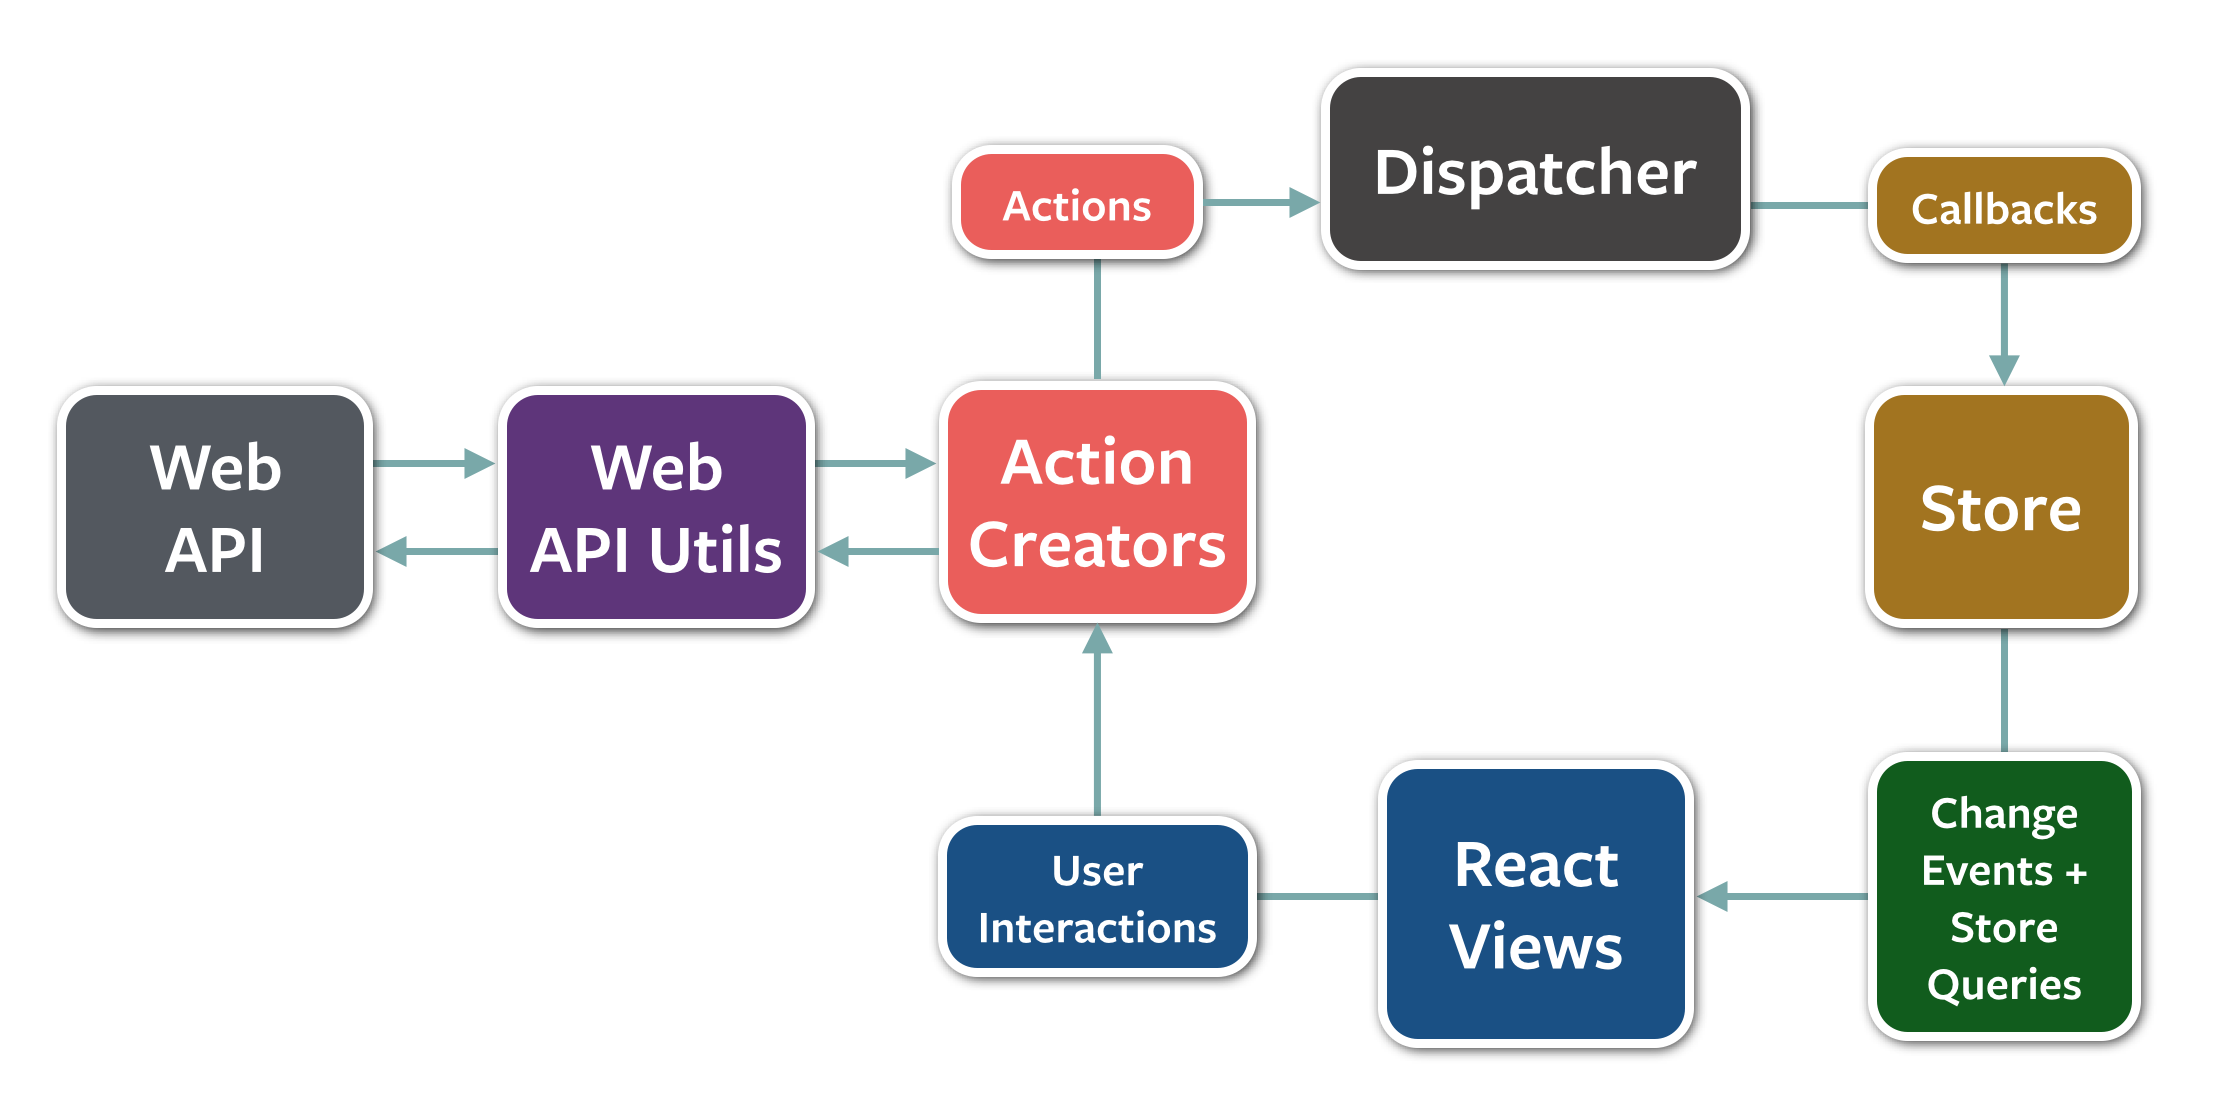
\includegraphics[width=.9\textwidth]{res/fig/flux-diagram-white-background.png}
  \caption{Rappresentazione del flusso unidirezionale dei dati in un'applicazione React con Flux}% % TODO: add figure reference
  \label{fig:flux}
\end{figure}

Come è possibile vedere in~\Cref{fig:flux}, la struttura è composta da quattro entità principali:
\begin{description}
  \item[Store]
    Rappresenta il ``contenitore'' che incapsula lo \emph{stato} (del dominio applicativo e/o dell'interfaccia grafica).
    Ciascuno store agisce come \emph{single source of truth} (SSOT)
    e non permette di modificare direttamente i valori dello stato, ma solo tramite \emph{azioni} passate con un \emph{dispatcher}.
  \item[Dispatcher]
    Singolo oggetto che invia in broadcast come eventi le azioni agli store;
    gli store devono essere registrati per gli eventi che sono in grado di gestire all'avvio dell'applicazione.
  \item[View]
    Rappresenta la componente di interazione con l'utente;
    essa osserva gli store per aggiornarsi al variare dello stato e genera azioni sulla base delle richieste dell'utente.
    Sono possibili due tipi di view:
    \begin{description}
      \item[Presentation view] Non si collega né al dispatcher, né agli store, bensì comunica tramite \emph{proprietà} definite alla costruzione.
      \item[Container view] Si collega al dispatcher e/o agli store, reagendo agli eventi e/o generandoli.
    \end{description}
  \item[Action]
    Oggetto semplice e immutabile che contiene tutte le informazioni necessarie per modellare un'interazione con lo stato.
    Possono essere generate dalla view o da API web esterne, ma sempre attraverso un \emph{action creator}.
\end{description}

Il flusso informativo avviene dunque in una singola direzione e tramite callback;
questo garantisce le seguenti proprietà:

\begin{description}
  \item[Asincronismo]
    Per come funziona il motore che interpreta JavaScript, ciascuna callback è eseguita al ciclo successivo, non bloccando l'esecuzione attuale.
  \item[Consistenza di rappresentazione]
    Essendo ciascuno store unico per l'intera applicazione, lo stato rappresentato dovrebbe essere unico indipendentemente dalla pagina attuale.
  \item[Disaccoppiamento]
    Essendo lo store esterno ai componenti grafici, essi risultano maggiormente disaccoppiati rispetto al dominio e più riusabili.
  \item[Determinismo]
    Essendo lo stato aggiornabile solo tramite azioni, non si hanno effetti secondari e l'applicazione risulta più facile da rappresentare come una sequenza finita di stati, agevolando anche la fase di testing.
\end{description}

\subsubsection{Redux pattern}

Il pattern Redux è una delle più popolari varianti del pattern Flux.

Redux\footnote{\url{http://redux.js.org}} è il nome della libreria JavaScript per la gestione dello stato che per prima ne ha definito un'implementazione.
Creata da Dan Abramov e Andrew Clark nel 2015 come implementazione alternativa a quella ufficiale del pattern Flux,
essa combina idee provenienti dal pattern \emph{Command}~\cite{10.5555/186897} e dall'\emph{architettura Elm} teorizzata con l'omonimo linguaggio~\cite{czaplicki2012elm}:
lo stato dell'applicazione è descritto da un singolo POJO (\emph{Plain Old JavaScript Object}) all'interno dello store e gli aggiornamenti avvengono tramite \emph{reducer}, funzioni pure di un'azione e dello stato corrente che generano un nuovo stato.

\begin{figure}[htbp]
  \centering
  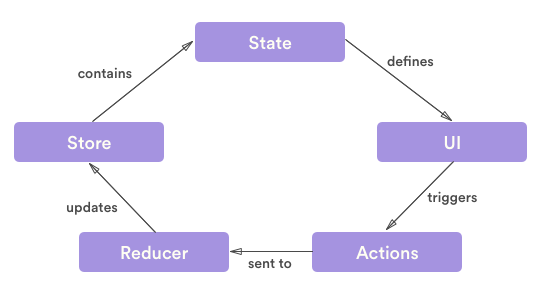
\includegraphics[width=.9\textwidth]{res/fig/redux-diagram.png}
  \caption{Rappresentazione del flusso unidirezionale dei dati in Redux}% % TODO: add figure reference
  \label{fig:redux}
\end{figure}

Secondo la documentazione ufficiale, la completa centralizzazione dello stato permette al sistema di essere completamente predicibile, permettendo il ``\emph{time-travel debug}'' tramite strumentazione integrata nel browser.
Inoltre, il non essere strettamente legato a un framework di rappresentazione e la possibilità di caricare middleware lo rendono estremamente flessibile.
